\documentclass[bsc,frontabs,twoside,singlespacing,parskip]{infthesis} 
\usepackage{graphicx}
\usepackage{listings}
\usepackage{url}
\usepackage{xfrac} 
\usepackage{booktabs}

\usepackage{courier}

\lstset{basicstyle=\footnotesize\ttfamily,breaklines=true}
\lstset{framextopmargin=50pt}

\graphicspath{ {images/} }

\begin{document}

\title{Text Driven Talking Heads}

\author{Iain Brown}
\course{Computer Science}
\project{Undergraduate Dissertation} 
%\project{Undergraduate Thesis} % AI%Psy
%\project{4th Year Project Report}

\date{\today}
%\abstract{The aim of this project is to build a head motion synthesizer for a lifelike animated avatar. The head motions will be predicted entirely from the text of transcribed speech with the aim of finding a mapping between the text and natural head motions. Unlike previous areas of research where the head motions are generated from recorded speech.}
\maketitle
%\section*{Acknowledgements}
%Acknowledgements go here. 
\tableofcontents

% ============================================================= %
\chapter{Introduction}

%The Introduction chapter should always provide a 'roadmap' to the report. Of course it should provide an introduction to the problem being considered, but it should also give some details of what you did - do not leave this to the conclusion. You should give forward references into the rest of the report - e.g., "In Chapter 2 how algorithms and heuristics are used to deal with approximate counting are discussed", "The design of the system is presented in Chapter 4", "In Chapter 3 the reasons for choosing to focus on the bounded-degree case of this problem are explained"
%

- Head motion is very important when it comes to human communication \\
- Dialogue is much harder to fully understand without the non-verbal information \\
- Generating Lifelike avatars in many applications, VR, video games, shopping assistant \\
- Realistic head motions are vital otherwise humans may feel weird interacting with an avatar \\
- Project aimed to create a system that synthesises natural head motions just from the text \\
- Without knowledge present in speech \\
- Using Various Natural Language Processing Techniques \\

% ============================================================= %
\chapter{Background Information}

\section{Human Computer Interaction}

Human Computer Interaction is a field of Computer Science in constant change. With the goal of enhancing Human Computer Interaction researchers have looked to the field of Embodied Conversational Agents, where an intelligent agent is mapped to a graphical animation or body to replicate the most natural of interactions: face to face dialogue. \cite{ecas} 

Embodied Conversational Agents have had been found to enhance the interactions with computers \cite{conv_agents} and researchers are perpetually improving systems in order to increase user satisfaction. One of the biggest benefits to using an ECA is that the interaction is of a social nature, being more familiar to humans and aids the systems perceived trust worthiness, allowing a richer interaction between the user and the computer. Also the intelligibility of speech produced in noise is also improved when a speaker's face is visible \cite{emotion_head_motion}, this means that because the user has a physical representation of the ECA they can more easily understand what the agent is saying rather than if it was just speech output. These results suggest that nonverbal gestures such as head movements play a more direct role in the perception of speech than previously known. \cite{vis_prosody}

There are some limitations to consider when talking about ECA's, mainly to do with what Masahiro Mori called the Uncanny Valley effect. Mori states that the familiarity with a robot or graphic representation of an avatar increases in correlation with the rise of human likeliness, but there is a distinct fall in familiarity before achieving a life-like human representation referred to as the Uncanny Valley which causes revulsion in humans. \cite{uncanny}

\begin{figure}[h!]
	\centering
	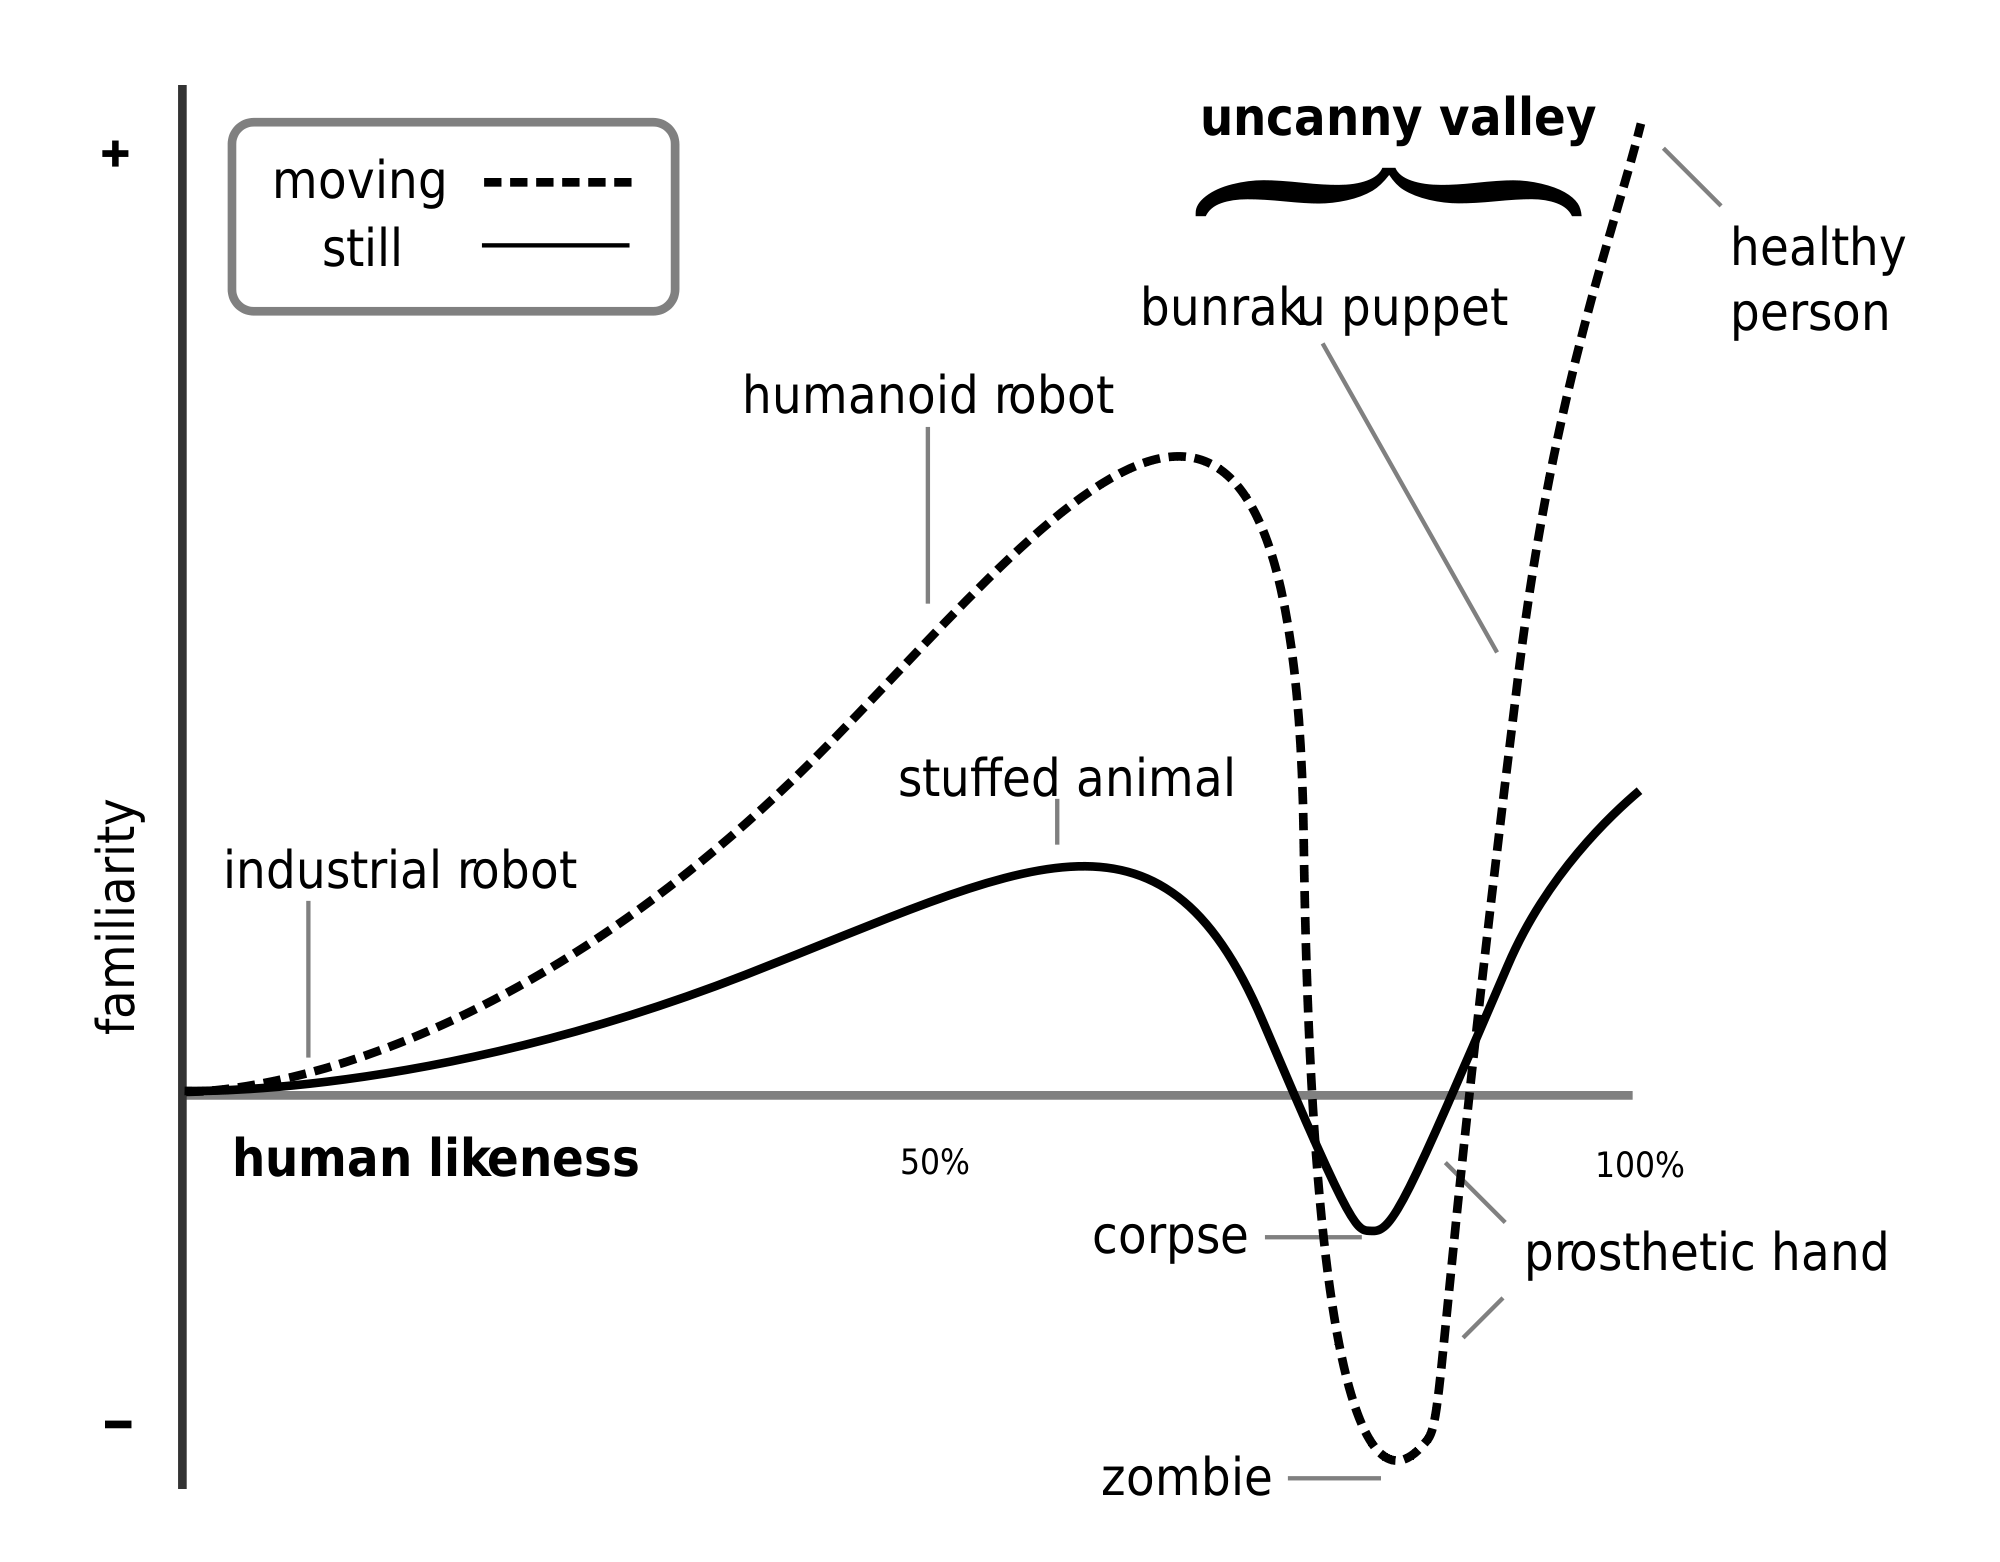
\includegraphics[width=0.6\textwidth]{uncanny}
	\caption{The Uncanny Valley effect}
\end{figure}

\section{Data and Task}

The task for the project was as follows: Using only text transcriptions of speech can we synthesise life-like head motions that seem realistic and natural to humans. The project aimed to investigate the correlation between head motions and the information present in speech unique to the speaker. The difficulty of the task comes from the lack of unique information about the speech, as we are only using the transcribed text. To tackle this we will be using a Text-to-Speech system called Festival.

\subsection{Data Recordings}

The data used for the project was data recordings from the Centre of Speech and Technology Research at Edinburgh University. The recordings consisted of optical motion capture sessions in which participants wore 4 reflective markers on their torso and a hat with 3 reflective markers. There were 7 V100:R2 cameras that tracked the reflective markers at a sampling rate of 100Hz. Participants were asked to read out transcriptions of fairy tales.

\begin{figure}[h!]
	\centering
	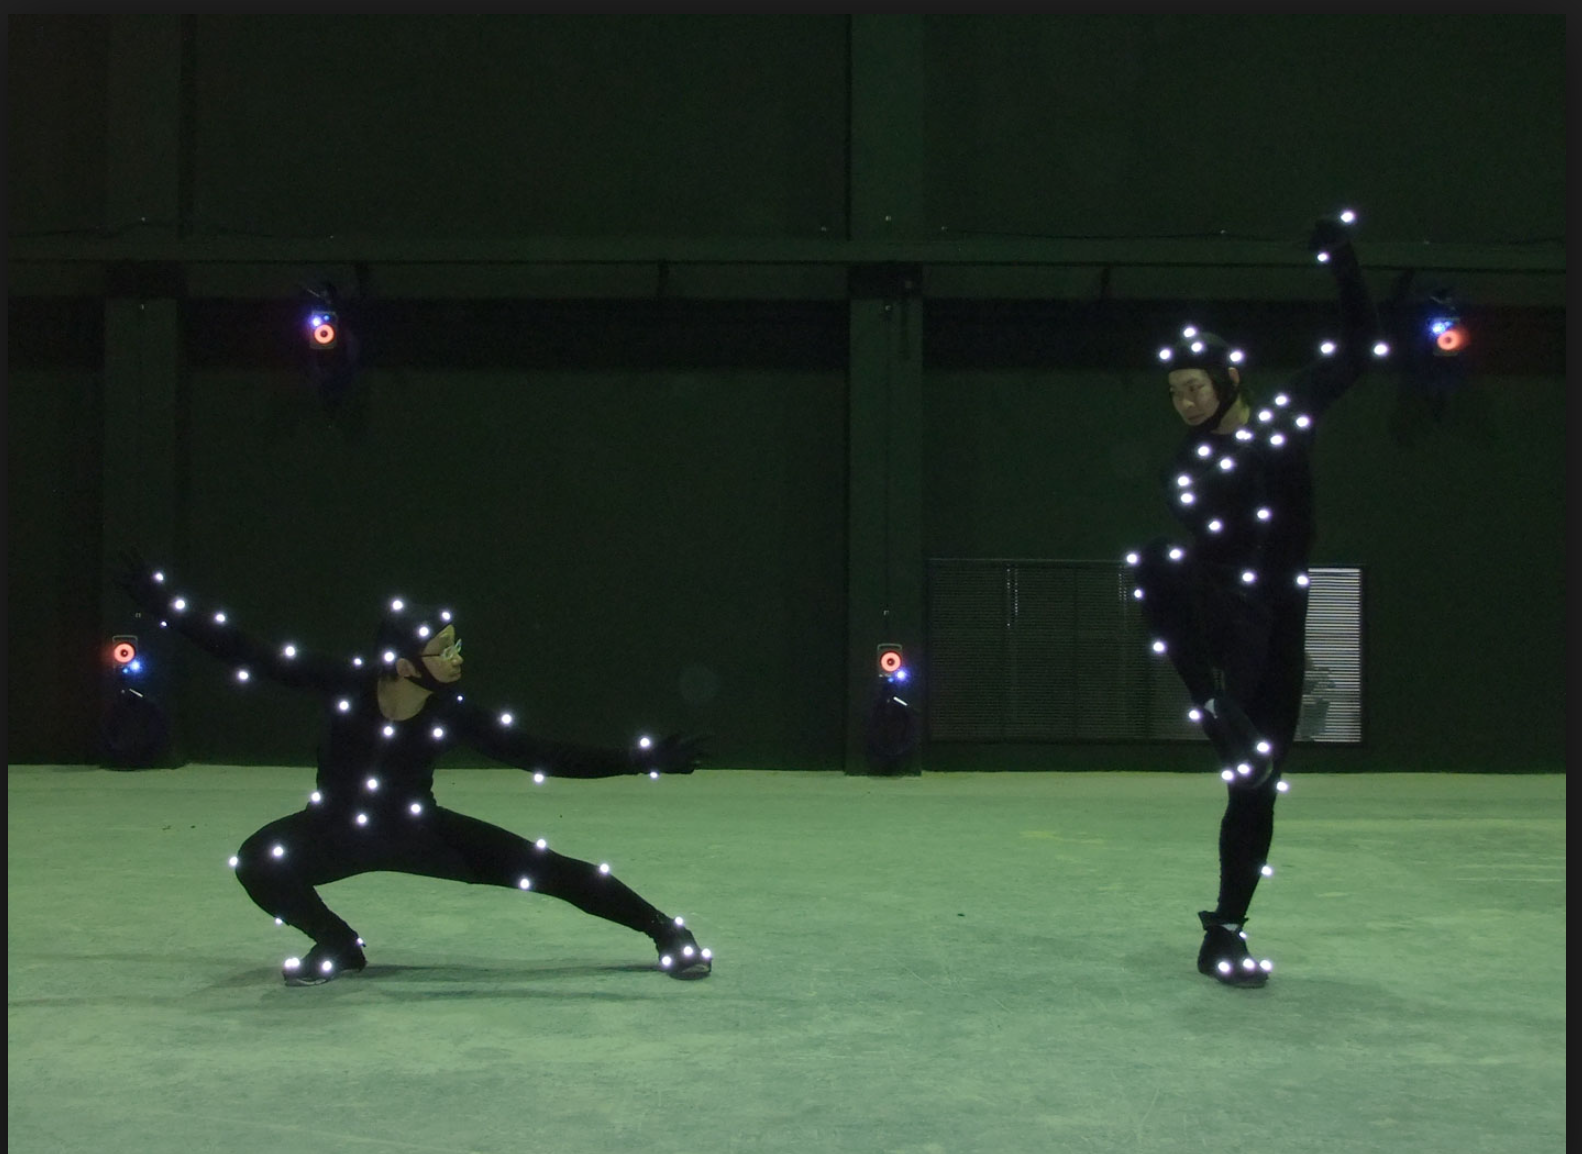
\includegraphics[width=.7\textwidth]{mocap.png}
	\caption{Setup of the mo-cap environment}
\end{figure}

\section{Euler angles}

Euler angles are three angles that represent the orientation of a rigid body in 3-Dimensional space, typically referred to as 'yaw', 'pitch' and 'roll'. Euler angles allows us to reduce the number of parameters normally used to represent rigid body orientation down to 3 parameters. It is a very popular method because of the reduced complexity and is commonly used in robotics and 3D animation. As the project focused on rigid head motions there was no translation taken into account when designing the 3D avatar head motions. This allowed the project to use Euler angles as the sole units of movement in the project.

\begin{figure}[h!]
	\centering
	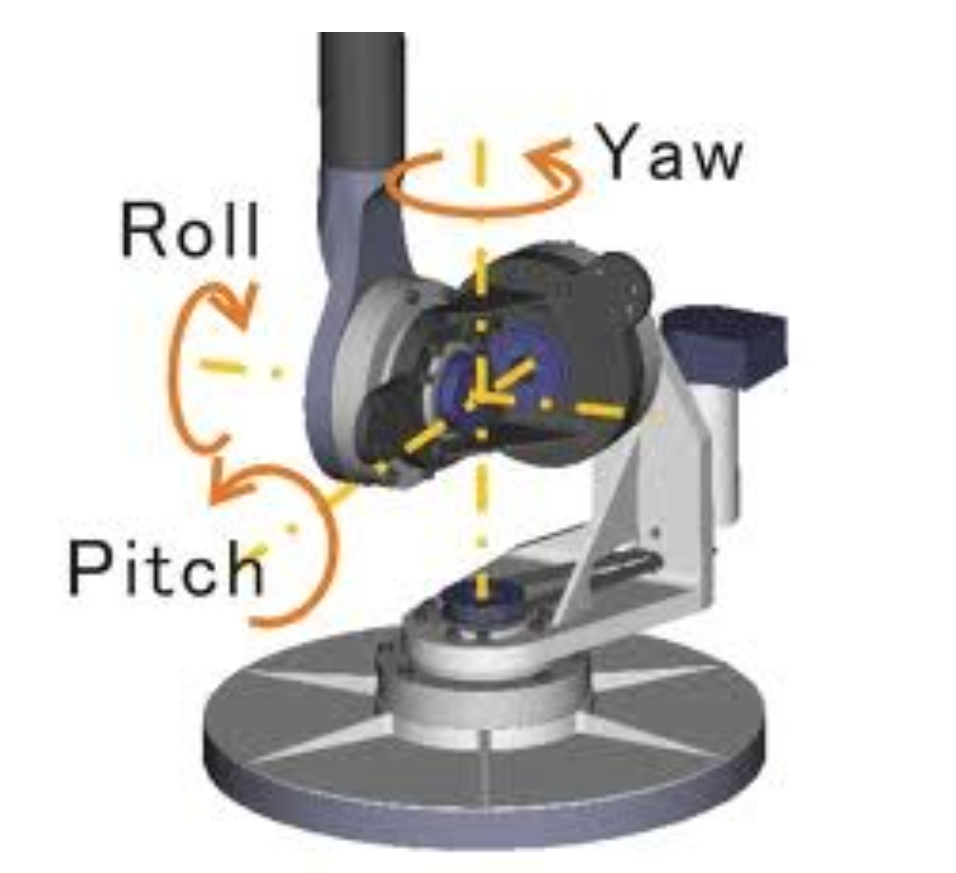
\includegraphics[width=.5\textwidth]{euler_angles.png}
	\caption{Euler Angles in Robotics}
\end{figure}

Euler angles do have some drawbacks. One of the most common issues animators experience with Euler angles is that different results can occur depending on the order of rotation. For example the rotation Roll x Yaw x Pitch will most likely have a completely different effect to the rotation Pitch x Yaw x Roll. \cite{quartionions} Another potential issue is the Gimbal Lock \cite{gimbal}. Euler angles were chosen because of their ease of use and these drawbacks were not an issue.

\section{Poser Animation}

3D animation and rendering software was used to visualise the generated head motions. The software used for this purpose was PoserPro 2012 by Smith Micro Software, a 3D animation tool with the emphasis on character creation and animation. PoserPro allows users to animate body parts of 3D characters and change their characteristic like rotation, translation and scale, meaning that the head of a character could be moved independently with ease.

With a scripting plug-in for Python called PoserPython, \cite{poser_python} allowing users to create scripts to manipulate objects and characters in the scene using Python. This was one of the main reasons for choosing PoserPro over other animation and rendering software like Blender. Poser also uses Euler angles as it's unit of rotation.

\begin{figure}
	\centering
		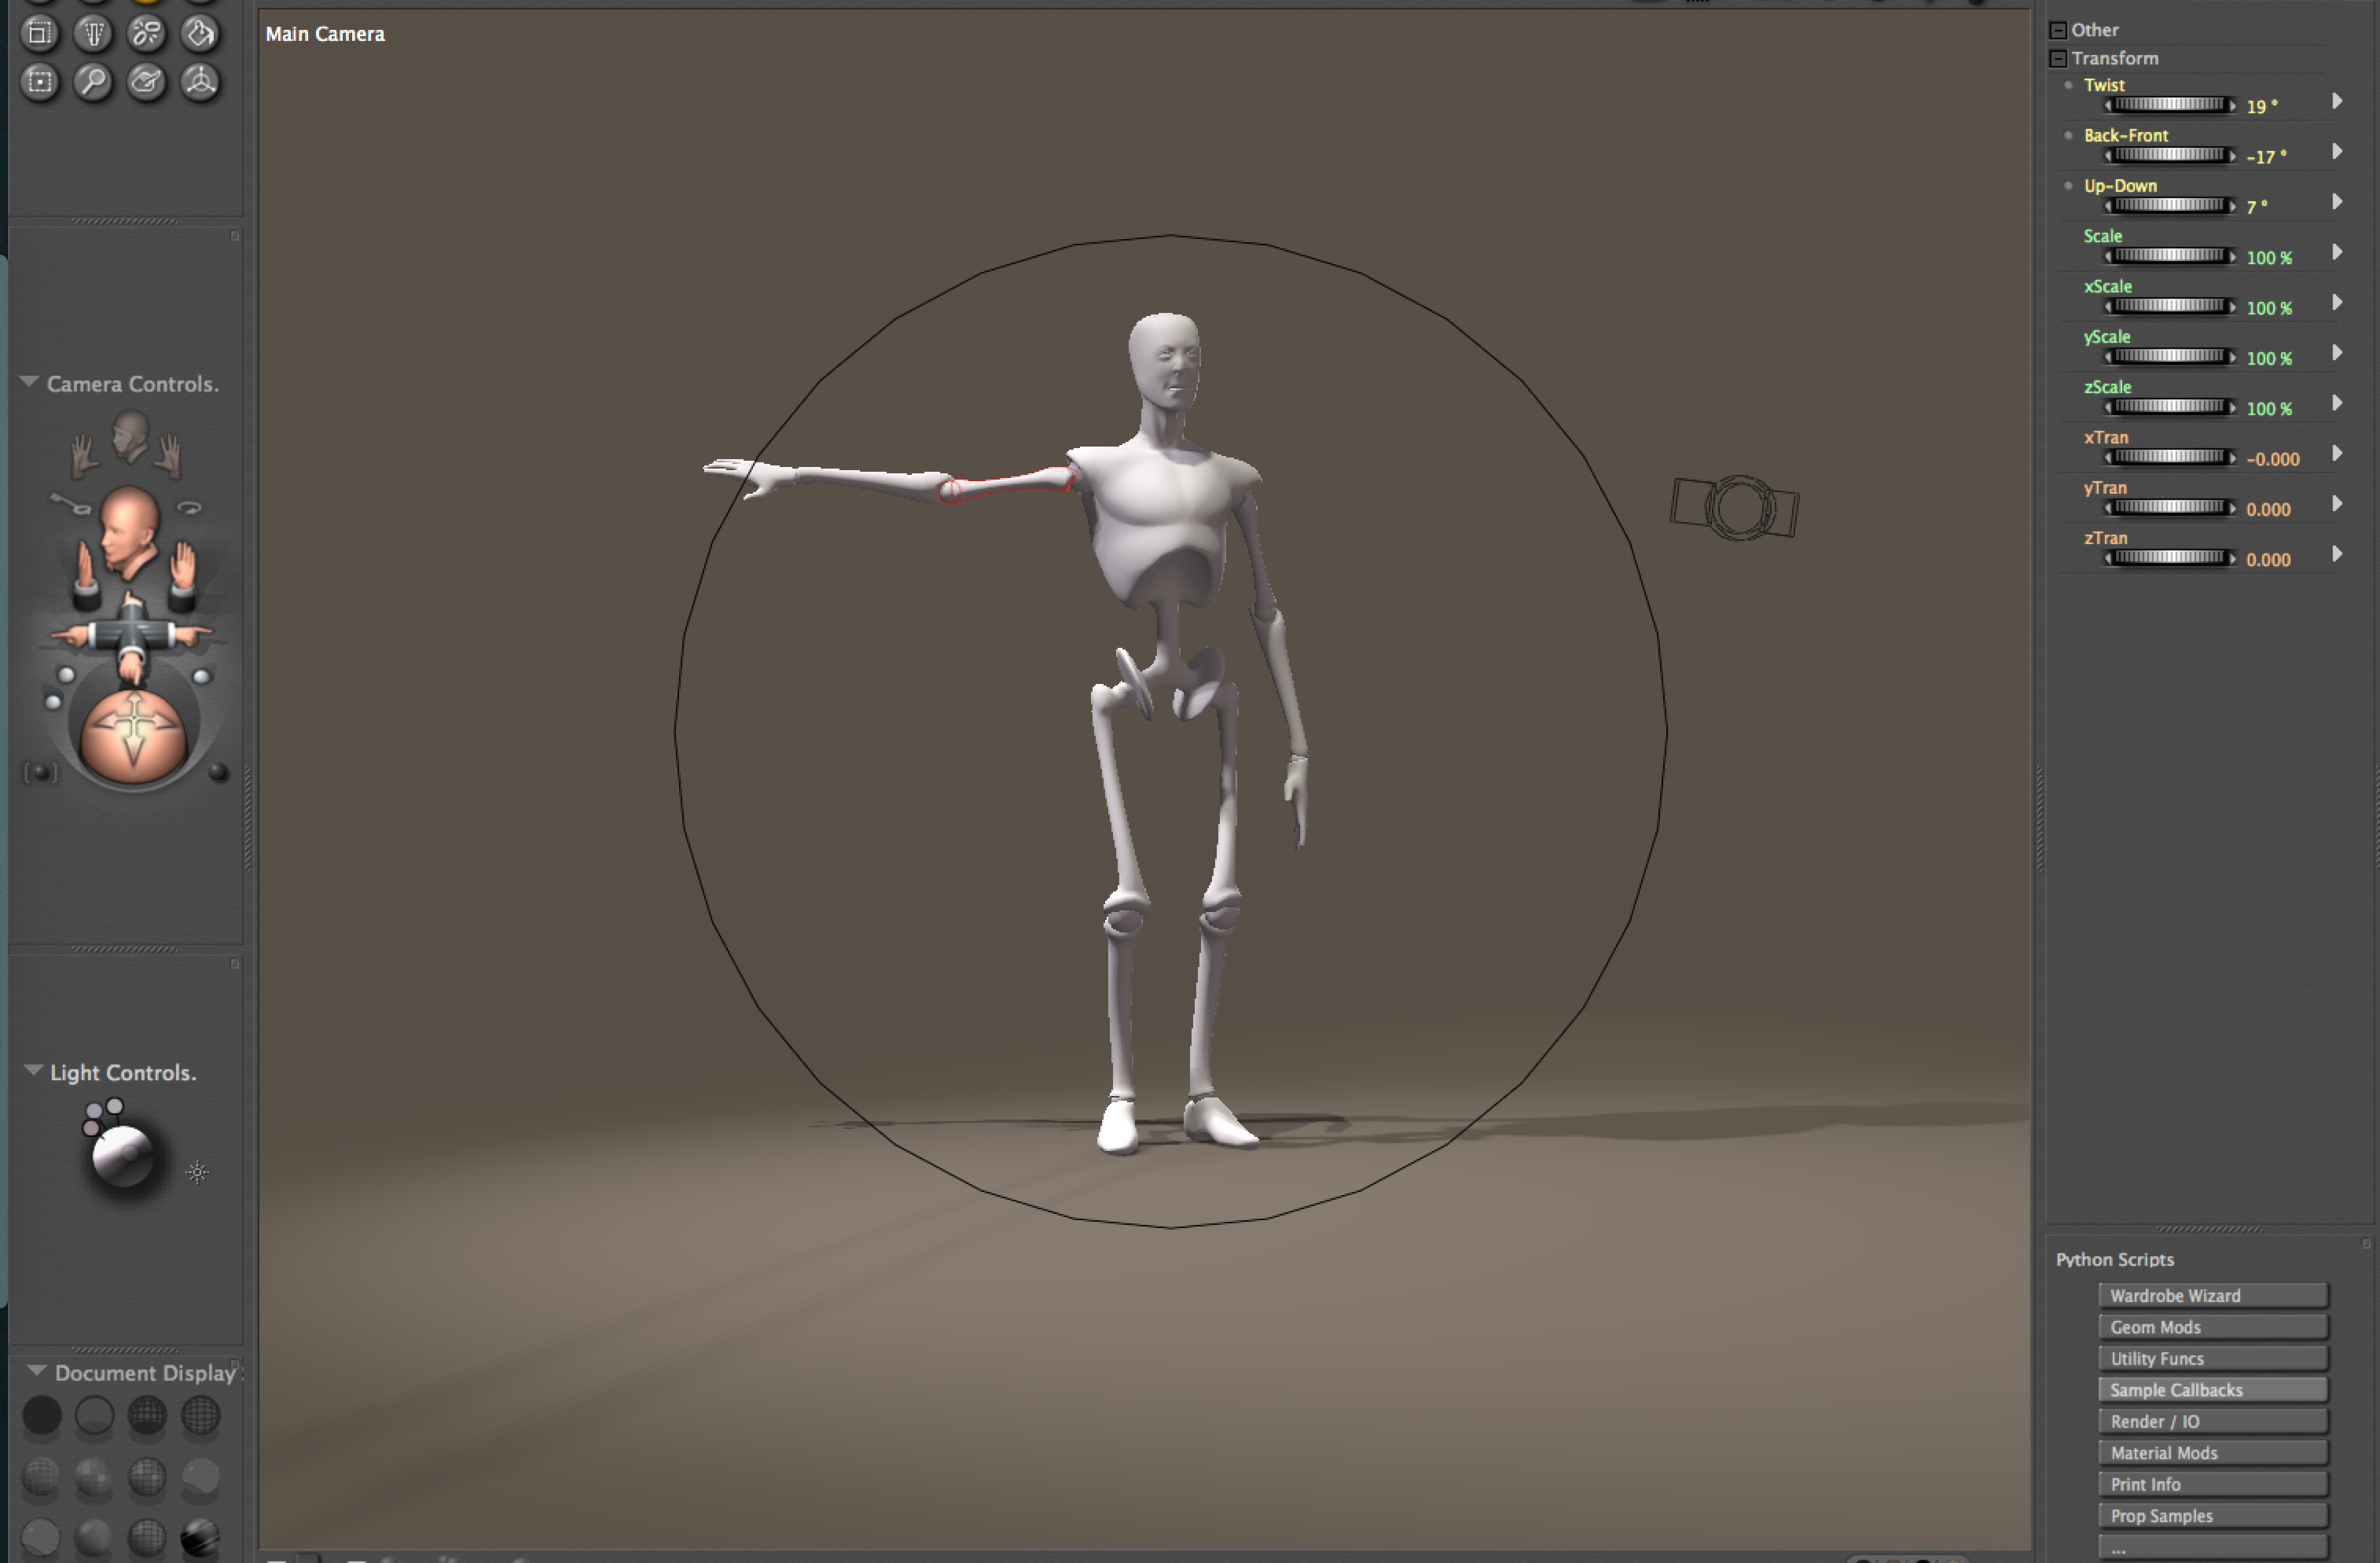
\includegraphics[width=1.0\textwidth]{poser.png}
		\caption{Overview of Poser Pro}
\end{figure}

%\section{Speech Features}
%
%F0

\section{Related Works}

Creating systems that are capable of synthesising life-life human motions as facial animations is a large area of computer graphics research due to it's rapid increase in demand in computer games, feature films and communications.

\subsection{Animation Synthesis Based on Speech}

There are a number of systems that use the paralinguistic information in speech to synthesise head motions and other facial animations using prosodic information like intonation. These approaches are data-driven approaches that use machine learning techniques in order to train models representing head motions and facial animations.

Hidden Markov Models are finite state machines with probabilistic state transitions that can be trained on data which are used in many machine learning based classification tasks \cite{hmms}. They are generative models of data and so can be used to synthesise similar data to what they have been trained on, because of this HMM's have been used in many of the systems as method of training data-driven systems \cite{puppetry}.  HMM's are very popular for data driven approaches as they eliminate the need to keep a large database of data as they can be trained fairly quickly \cite{expressive_speech_animation}. 

G. Hofer designed the Speech Driven Head Motion Synthesis system \cite{speech_driven_head_motion} in which a HMM based system was modelled to synthesise natural head motions by extracting important information from the speech such as the F0 values and the Mel-Frequency Cepstral Coefficients which provide a unique fingerprint of the speech derived from the Fourier transform and is commonly used in signal processing. This approach produced head motions that were within a 70\% accuracy to test data. A Ben-Yousse developed a system which improves upon the previous Speech Driven system by using articulacy features extracted the speech\cite{artic1} to synthesise head motions.

Similarly C. Busso designed a system to synthesise head motions using using speech by training HMM's on data. \cite{busso_rigid} The system generated discrete vectors for the head notions and applied interpolation as a form of smoothing to create realistic head motions. The system showed that HMM's were capable of capturing the relationship between head motions and speech data.

Systems have also been developed that aim to synthesise facial movements to express emotions, rather than just synthesising natural head motions. Y. Cao designed the Expressive Speech-Driven Facial animation system  \cite{expressive_speech_animation} in which they used similar machine learning techniques to discover the mapping between F0 and head motions. The system takes in recorded speech, extracts key features such as the phoneme sequence and spectral envelope, performs emotion analysis and executes a graph search through their Anime data structure, designed to combine utterances with their recorded head motion. As outlined in the paper the system needs a lot of training data which is expensive to record. 

\subsection{Text Analysis for Facial Animation}

All of the approaches to facial animation have used speech data as their primary source of information, but there are also systems in place that perform facial animation synthesis with just text as their primary source of information, without the need for speech. As speech is not always available these system use natural language processing techniques to analyse the text in order to synthesise facial animations like head motions of lip motions.

"May I talk to you? :)"  \cite{may_i_talk_to_you} is a system that was designed to synthesise facial animation from just the text. The system uses a Text to Speech system which analyses the text and generates information about the text such as accents and pauses in order to synthesise non-verbal speech related facial expressions like lip motions and head movements. The system also allows the input of emoticons to indicate emotions (text representations of facial expressions) to dramatically alter the synthesised facial animation. 

Similar to the previous system, much research has gone into synthesising lip motions solely using the text. In T. Masuko's paper  \cite{lip_motion}, their team designed a data driven system using Hidden Markov Models to accurately generate lip motions from text for Japanese. The approach is similar to those outlined in the previous section that also use HMM's.

\section{Subjective Evaluation Approaches}

This project used subjective evaluation to determine how natural the synthesised head motions were, according to humans. This was important because the project aimed to synthesise head motions that were natural for humans in order to be used in Embodied Conversational Agents, so humans had to deem the head motions as natural.

Subjective analysis is problematic due to evaluation being based on feelings and not measurable facts. This is a problem because 'feelings' and the evaluation itself can vary widely, even in the same person due to external factors like the time of day. Care must be taken when designing subjective evaluation environments and tests to mitigate variability and many tests need to be conducted in order to account for the this. 

There are many different approaches to performing subjective analysis, each with their pros and cons. 

\subsection{Preference Tests}

Preference tests are very simple to conduct. A participant is presented with two video samples and asked "Which do you prefer?". This is an example of an AB test using two samples. AB testing is very simple to conduct and so is very common when evaluating samples of video or audio. However, if there were more than two samples then the time needed to evaluate all samples would be significantly higher as each pair combination of samples would need to be conducted. ABX testing, \cite{abx_testing} is where the participant is shown three videos (A, B and X) and is asked 'Is X more like A or B'. This approach is an alternative to AB but runs into the same issues with time constraints.

Preference testing is suitable for evaluating a small number of samples, simple to conduct and produces easy to understand results. It's main drawback is the time needed to perform the evaluations which increase quickly as the number of samples increase.

\subsection{Mean Opinion Score - MOS}

When evaluating 'Naturalness' where the concept is not so clearly defined, the MOS test is commonly used as the method of subjective analysis. \cite{mos}

The Mean Opinions Score (MOS) is a test to obtain the user's subjective measurement of quality in relation to a particular feature or concept. Generally, users will be asked to rate something on a numerical scale like 1 to 5, 1 being the worst or 'bad' and 5 being the best or 'very good'. This method is fairly trivial and is a very common form of subjective evaluation due to is ease. Results from MOS testing are easier to analyse than preference tests due to their values being numerical.

\subsection{MUSHRA : Multiple Stimuli with Hidden Reference and Anchor}

Multiple Stimuli with hidden Reference and Anchor is another methodology for subjective evaluation more commonly referred to as MUSHRA \cite{mushra}. In a MUSHRA test, the subject is shown multiple stimuli are available at the same time which the subject can switch between and go back to and then gives a rating from 1-100 depending on how the subject was asked to rate the stimuli. Anchors are used in the evaluation, hidden in the test as one of the stimuli to serve as a reference point for each candidate. These anchors are supposed to score highly on the test. Subjects that score these particular stimuli are usually deemed as unreliable. Typically a MUSHRA test is used for evaluating audio quality \cite{mushra_bbc} where the subject is given 5 audio clips to listen to and rate the quality on a scale of 1 to 100.

The main advantage of MUSHRA over the other two method of subjective evaluation is that many different stimuli can be evaluated at once meaning MUSHRA can scale up the number of samples easily with little change in the time taken. This also means that MUSHRA requires less participants in order to obtain significant results in comparison to MOS even though they are similar in their design.

% ============================================================ %

\chapter{Text-Driven Head Motion Synthesis}

The goal of this project was to develop a system that was capable of synthesising life-like, realistic head motions from transcribed speech. This project aimed to developed a system that was capable of synthesising head motions given just the text. In order to to this hypotheses about the relation of head motion events and speech content were introduced. The system built on these hypotheses, linking them together in order to synthesis the final head motions. Text itself is very limited in information, so in order to have richer input data the transcribed text would be passed through a Text to Speech system which would apply natural language processing techniques in order to synthesise speech. 

\section{Hypotheses}

It was  found that when two people have a conversation, head motions are more prevalent in the dialogue if the two people do not have a close relationship. \cite{first_paper} In dialogue the nod is commonly understood as a gesture of affirmation and agreement. A possible explanation for this effect could be that because there is no pre-existing relationship humans subconsciously overcompensate their head motions as a method of positive reenforcement to aid in building a foundation for this new relationship. In the context of Embodied Conversational Agents the system aimed to synthesise head motions that made the interaction between the user and the ECA as natural as possible in relation to head motions, to incorporate this hypotheses into the system the main head motion should primarily be a nodding motion and head motions should overcompensate similar to an interaction with a new person with the aim of making the interaction feel more like a face to face conversation and provide a  more comfortable experience.

\subsection{Prosodic Features}

Prosody is the rhythm, stress and intonation of speech. As english is the language domain for the project and english is a stress timed language \cite{stress_timed}, prosodic features in speech are very important to the meaning of speech and can change the meaning of the underlying text.

Head motions correlate strongly with prosody present in speech \cite{vis_prosody}. My first hypothesis relates to the rate of change of the fundamental frequency present in the synthesised speech. This is indicated in the Festival output as values around 120 Hz for male voices and 210Hz for female voices \cite{f0_values}. Sudden changes in the frequency should be reflected in head motions. For example in the intonation falls the head should lower accordingly \cite{Kendon}.

\subsection{Phrasing}

Phrasing plays a huge role in how something is said. It has been found that nodding head motions frequently occur at the end of phrases or at strong phrase boundaries, especially if the speaker is confident in what they are saying. \cite{ishi2008}. 

\subsection{Sentiment Analysis}

Sentiment analysis is a popular area of natural language processing. It is often used to gauge reviews for products\cite{sentiment_online} and films\cite{sentiment_films} due to the availability of data and ease of tagging the reviews as either positive or negative.

Sentiment or emotion in speech has various effects on head motions. In a study It was found that the absence of head motion can be easily identified as 'neutral' emotion. \cite{emotion_head_motion} whereas participants in the study found it difficult to differentiate between head motions that were typical of 'happy' and 'sad' emotions. This study shows that emotive analysis on the text should be treated as an 'intensifier' of the underlying head motions derived form other areas of the text rather than altering the head motions to fit an emotion.

Negation is very commonly associated with head shakes \cite{head_shaking}. For example, it is very common for people to respond to a question by shaking their head and saying "No". The head shake is strongly associated with negation. Sentiment analysis can be used to determine wether a sentence is positive or negative, however there are many other factors that relate to head shakes. Kendon states that head shakes can be used as an affirmation \cite{kendon} in many positive sentiment sentences. 

For example in the sentence "I have never saw anything more beautiful in my life" has a positive sentiment as the subject is talking about something beautiful but the subject will shake their head on the word 'never' to enforce the positive affirmation. As pointed out in another paper \cite{negative_sentiment} negation statements are very ambiguous and sentiment alone cannot capture the overall meaning and that the lexical structure may play a large role.

\subsection{Text Content}

There are two types of gestures that relate to speech. \cite{lexical_gestures} The first are motor movements which are typically simple, brief, repetitive and have a high correlation with prosodic features. The other type are lexical movements, gestures that help the speaker mentally perform lexical lookups subconsciously. These gestures are very different to motor movements and are much longer, more complex and relate more to the lexical information in the speech. To portray these ideas in this project, unique words that are not common should cause the avatar to tilt their head. This is similar to the theory that eye movements can aid with memory recall. \cite{eye_movements}

\section{Text analysis with Festival}

Festival applies various Natural Language Processing techniques to the text to generate information  so that it can synthesise speech.  There are many steps in this pipeline, each adding a little bit more information to the text before Festival can then apply signal processing to generate audio. 

The first stage in the Text to Speech pipeline is the text processing. Festival breaks the text up into more suitable units for processing, for example expanding abbreviations. Then Parts-of-Speech tags are assigned to the units, these POS tags indicate what type of word it is and how it relates to the overall structure of the sentence allowing for phrase break prediction and are represented as a series of capital letters. For example "NNP" is a pos tag indicating that the word is a singular proper noun. POS tags are useful for the project to determine which words are the subject of the utterance and show where the emphasis should lie in the synthesised speech, which will be reflected in the synthesised head motions.

Phrase break prediction assigns a break strength to each unit, which highlights where the phrases are in the sentences. Phrase break predictors are usually taggers trained on annotated data and are accurate. This is shown in Festival as a series of tags with their assigned values. The 'pbreak' indicates what level of break has been assigned to this word, for example BB for a big break, B for a normal break or NB for no break.

\begin{lstlisting}
	pbreak_index 0 ;
	pbreak_index_score 0 ;
	pbreak B ; 
	blevel 3 ; 
\end{lstlisting}

As outlined in the hypothesis section, head motions frequently occur at the end of phrases, where there will be a strong break strength like a big break or normal break. The phrase break value will be very useful to determine these breaks to synthesise head motions.

Festival generates pronunciations by performing syllabification, breaking the sentences and words into syllables and looking up phonemes in a lexicon to determine their pronunciations. Using this information the system can generate ToBi markers \cite{tobi}, a way of symbolically representing intonation. These symbols are useful as they are conceptually easy to understand and reduce the number of parameters needed to represent intonation. A typical marker will indicate the tone in terms of two letters : 'L' for a low intonation and 'H' for a high intonation, these can be combined to represent a rise from low to high intonation such as 'L-H\%' or vice versa.  This means that sudden rises or falls in intonation can be identified easily when synthesising head motions. 

Similarly to phrase break predictors, Festival uses duration predictors that have been trained on annotated data using classification and regression trees to produce duration information for each phoneme.

Now that the system has a linguistic specification of the sentence like the phone sequence, phone duration and pitch contour signal processing can be performed to generate the final speech output.

\begin{figure}[h!]
	\centering
	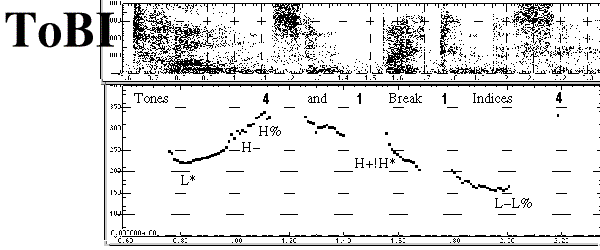
\includegraphics[width=0.8\textwidth]{tobi.png}
	\caption{ToBi Markers}
\end{figure}

\section{Head Motion Synthesis System}

\begin{figure}
	\centering
	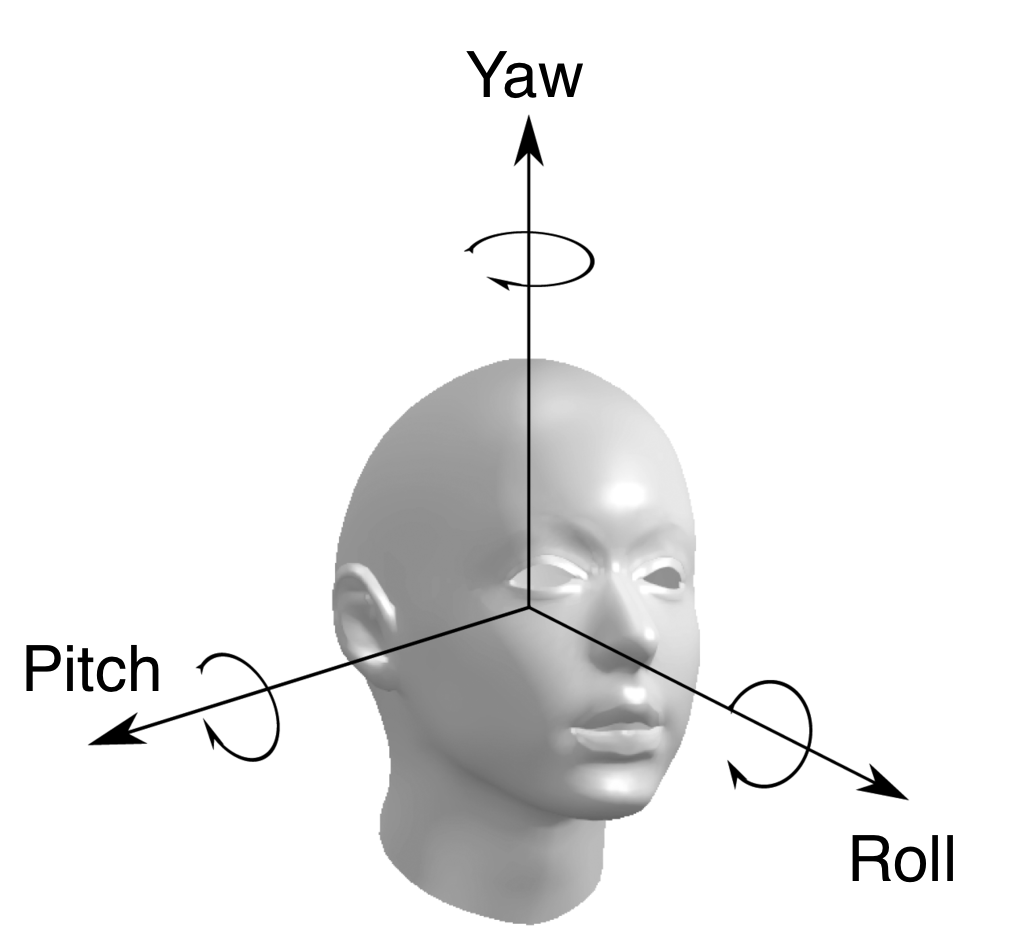
\includegraphics[width=0.6\textwidth]{head_with_euler.png}
	\caption{How Euler Angles affect head rotation.}
\end{figure}


\subsection{Outline}

\begin{figure}
	\centering
	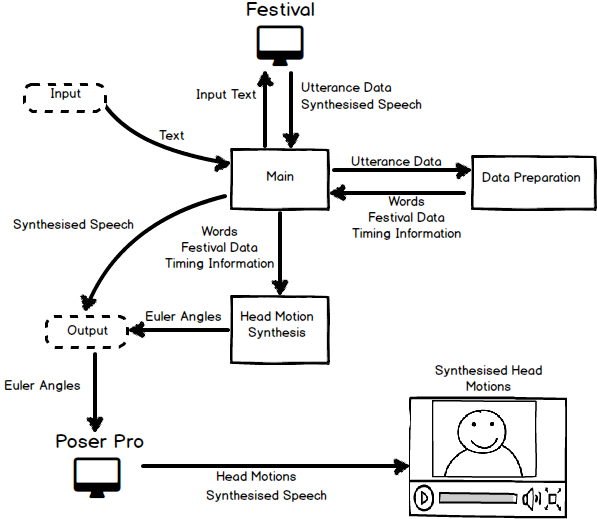
\includegraphics[width=0.8\textwidth]{system.png}
	\caption{Outline of System Architechture}
\end{figure}

\subsection{Basic}

\subsection{Random}

\subsection{Rule Based}

% ============================================================= %
\chapter{Implementation}

The system was implemented using Python, a high-level programming language widely used for many purposes including scripting and large scale software development. Python was the clear choice for many reasons including powerful libraries such as NLTK (Natural Language Toolkit) \cite{nltk} and it's scripting compatibility with Poser. 

The initial difficulty of the project was that there were a lot of individual components to tie together, like Festival and Poser. The subprocess module in Python allows the script to spawn new processes, connect to their input and output and retrieve their return codes. This was invaluable in the project as it allowed the Python script to call Festival with parameters that could change with each run.

\begin{lstlisting}
fest_location = DIR+'preparation/text2utt.sh'
festival = subprocess.Popen(
		[fest_location,text_file], 
		stdout=subprocess.PIPE
		)
utterance = festival.stdout.read()
return utterance
\end{lstlisting}

The data received from the Festival output was a large block of text containing information about the utterance it had processed (See Figure 4.1). This data was fed into a text processing module implemented from scratch to extract the important information regarding the utterance and build a dictionary using these elements to link the individual words with their properties like parts-of-speech tags and phrase break strength.

\begin{figure}
%	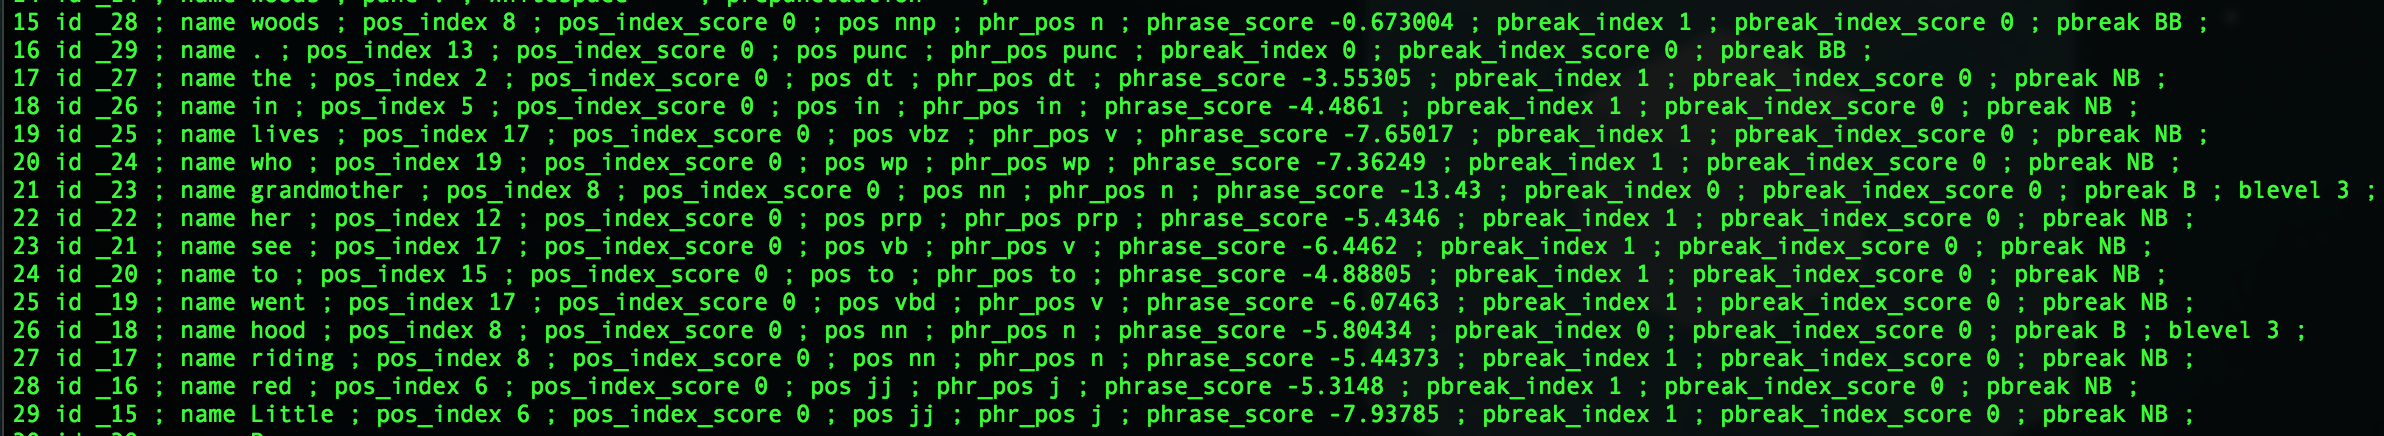
\includegraphics[width=1.0\textwidth]{festival_output.png}
	\begin{lstlisting}
		id _23 ; name grandmother ;
			pos_index 8 ;
			pos_index_score 0 ;
			pos nn ; 
			phr_pos n ; 
			phrase_score -13.43 ; 
			pbreak_index 0 ; 
			pbreak_index_score 0 ; 
			pbreak B ; 
			blevel 3 ; 
	\end{lstlisting}
	\caption{An Excerpt from the festival analysis output}
\end{figure}


Normally Festival is run as an interactive interface. The system used a LISP script called "text2utt.sh" that came with the installation, allowing it to run batch commands in "Text to Speech mode" without entering an interactive state. This was perfect for the project but in order to extract duration information correctly and save the outputted speech to audio files the script had to be altered by adding in the following code. 

\begin{lstlisting}
1. (utt.save.words utt outfile 'est_ascii) 
2. (save_waves_during_tts)
\end{lstlisting}

The line of code (save\_waves\_during\_tts) meant that Festival saved all synthesised speech to wave files. An issue that raised from this was that it generated an audio file for each sentence, which was not suitable for the Text-Driven Talking Heads System. This problem was solved by implementing a function in the preparation stage called \"combine\_audio\_files\" which created a new file that was the concatenation of all the sentences. This was a suitable solution as the produced output sounded quite natural.

The Poser Script setMotion.py was taken from another Project that used Euler Angles to rotate a character's limbs, the only alterations made were to set he active body part to the head, add the speech to the scene and to load in the output of the Head Motion Synthesis by hardcoding the name and location of the output file.

The head motion synthesis was developed as three separate modules, increasing in complexity and building on what was successful from the previous head motion synthesis methods.

\section{Basic System} 

\subsection{Trignomietric Functions}

\begin{figure}
	\centering
	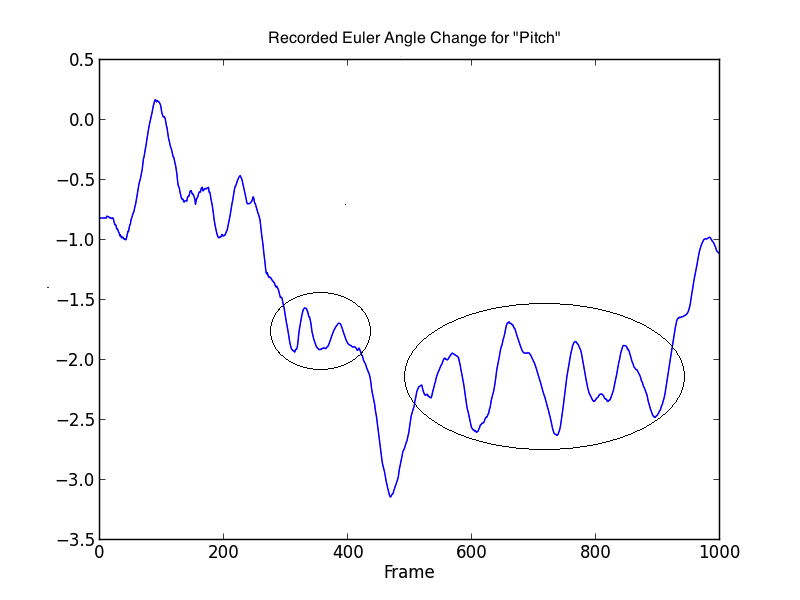
\includegraphics[width=0.8\textwidth]{euler_change.png}
	\caption{Visualisation of Euler change from data recordings}
\end{figure}

As outlined in chapter 3 the most common occurring head motion in dialogue is the nod which was reflected in the analysis of the recorded motion data. This implementation of this hypothesis is the baseline system. It aimed to synthesise a natural nodding motion distributed across the length of the utterance.

The nodding motion is a smooth repetitive oscillation of the head along one axis and visualisation of the data recordings (Shown in figure 4.2) shows that there are large sections of data which are very similar to a sine wave's oscillation so the first system used the trigonometric sine function as it's model.

The file basic\_predict.py takes in the dictionary containing all the information retrieved from festival and calculates the number of frames needed for the output rotations and calculates the angle change per frame so that the motion from the first frame to the last frame represents one complete oscillation of the sine formula.

The prediction system adds the rotation information for each Euler angle to the dictionary of utterance data and returns said dictionary. That dictionary is then passed to output.py, which is a generic function that also accepts the utterance dictionary and a filename so that there was no need to re-implement and output function for each system and also allowed for comparison between the systems without necessarily saving them to file allowing rapid prototyping.

As mentioned, the basic system only took one axis into account and so only altered the "Roll" Euler angle. This system although simple, showed promising results and provided the workflow to have a working system that synthesised head motions, saved them into a .head file containing the Euler angle change for each frame which can be read in by the PoserPython script and assigned to character to be rendered out.

\section{Random System}

The basic system itself produced a natural nodding motion, but after having compared the output of the basic system with the motion recordings, especially comparing different individuals speaking the same sentence there were a low correlation between what the participants were saying and how their head movements changed. To represent this finding the second system moved away from trigonometric functions.

\subsection{Discrete Head Motions}

The next system was designed to assign random discrete numbers to each word in the utterance for all Euler angles and apply a form of smoothing to make the random assignment seem smooth and natural even though it was completely random. 

Each word in the utterance was assigned Euler values, ranging from -10 to +10 for "Roll" and -5 to +5 for the "Pitch" and "Yaw" as the "Roll" relates to nodding motions which are found more frequently head motions. The random function was implemented using Python's random library.

\subsection{Smoothing}

To synthesise smooth head motions between random points multiple interpolation algorithms were considered. Spherical Linear Interpolation (Slerp) was the first that was considered and was already used in similar research \cite{rigid_head_motion}. There was difficulty when trying to implement Slerp due to the choosing Euler angles as the unit of rotation. Euler angles are difficult to apply interpolation \cite{quartionions}, Slerp commonly uses Quartinions which are more complex. Another method of interpolation which was derived from Slerp which was considered was the Bezier Interpolation algorithm, invented by Pierre Bezier a french mathematician was much simpler to implement than Slerp.

A recursive Bezier function was implemented which, given a list of points return a formula representing the a smooth interpolation between said points. Unlike Slerp, Bezier's smoothing algorithm doesn't take the interpolated line to the given points which works well given this scenario. It helped to smooth out the randomness and generate natural motions. (Figure 4.5)

\begin{figure}
	$$ B_{P_0}(t) = P_0 $$
	$$ B(t) = B_{P_0P_1..P_n}(t) = (1-t) B_{P_0P_1..P_n-1}(t) + tB_{P_1P_2..P_n} (t)$$
	\caption{Recursive Bezier Definition} 
%	\centering
%	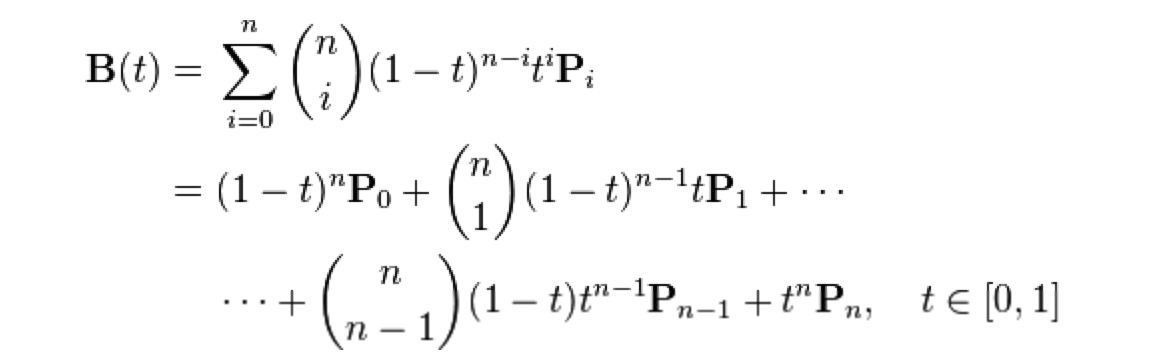
\includegraphics[width=0.8\textwidth]{bezier_general.png}
%	\caption{General Form}
\end{figure}

The random system calculated a Bezier function for each of the Euler angles and returned a dictionary containing the Euler angle change for each frame of the animation which was passed to output.py.

%\begin{figure}
%	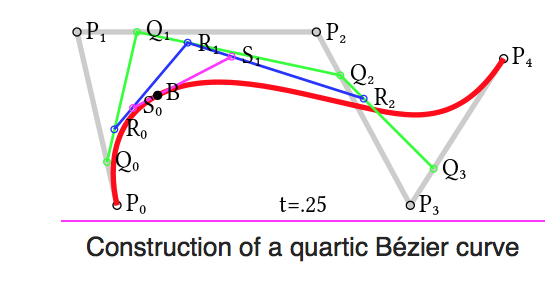
\includegraphics[width=1.0\textwidth]{bezier_example.png}
%	\caption{Example of Bezier}
%\end{figure}

\begin{figure}
	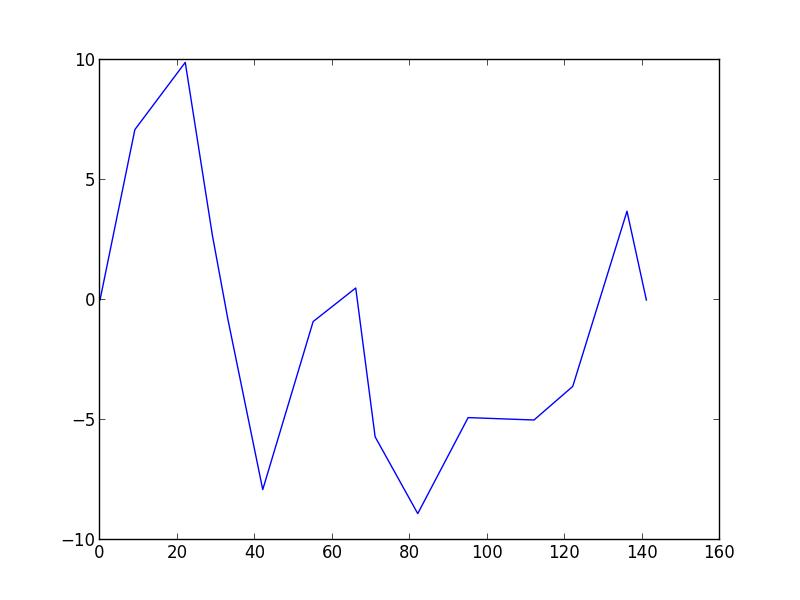
\includegraphics[width=.5\textwidth]{figure_1.png}
	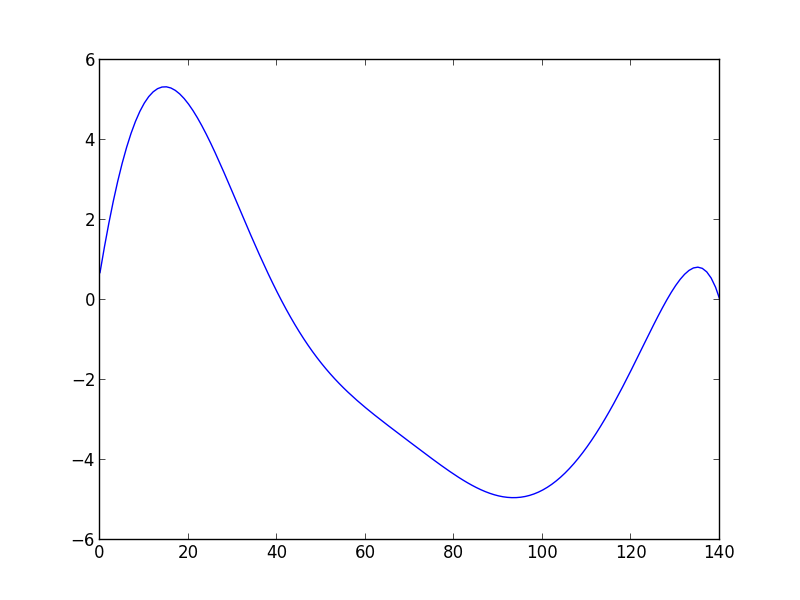
\includegraphics[width=.5\textwidth]{figure_2.png}
	\caption{Applying Bezier Smoothing to the discrete points}
\end{figure}

\subsection{Introduction of noise}

The output of the second system when mapped to a character in poser showed promise, the motions were smooth and looked like they could have been recorded from actual participants, however the motions produced were deemed too smooth and approached the uncanny valley, looking unnatural.

To counteract this issue a probability based assignment was introduced which adds or subtracts a very small percentage with the purpose of adding noise to the output. This was done with the use of python's in built random library, functions in the library are based on the random() function which generates a random float uniformly in the range of 0.0 to 1.0. The values used for noise ranged from -0.01 to +0.01. The introduction of noise reduced the feeling of the uncanny valley in the initial results.

\begin{figure}
	\centering
	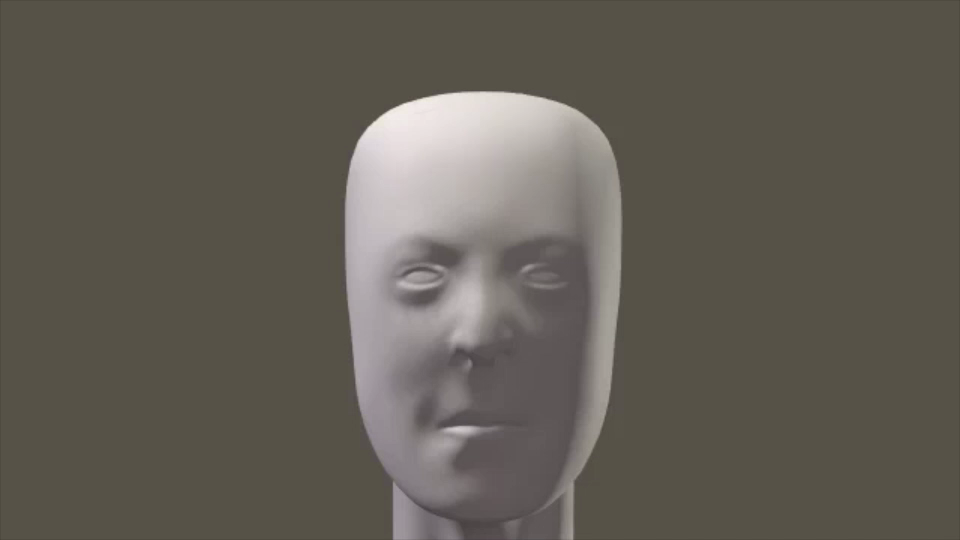
\includegraphics[width=.3\textwidth]{fightclub1.png}
	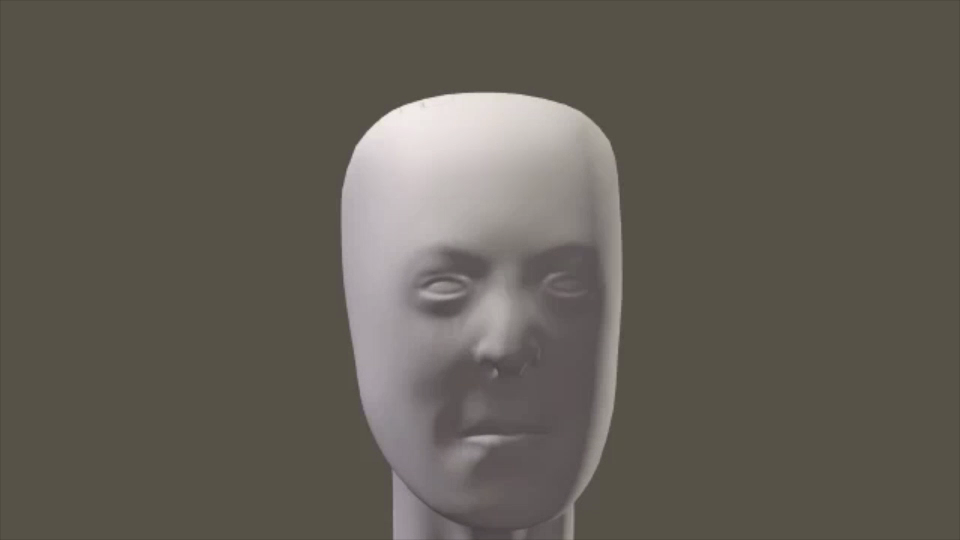
\includegraphics[width=.3\textwidth]{fightclub3.png}
	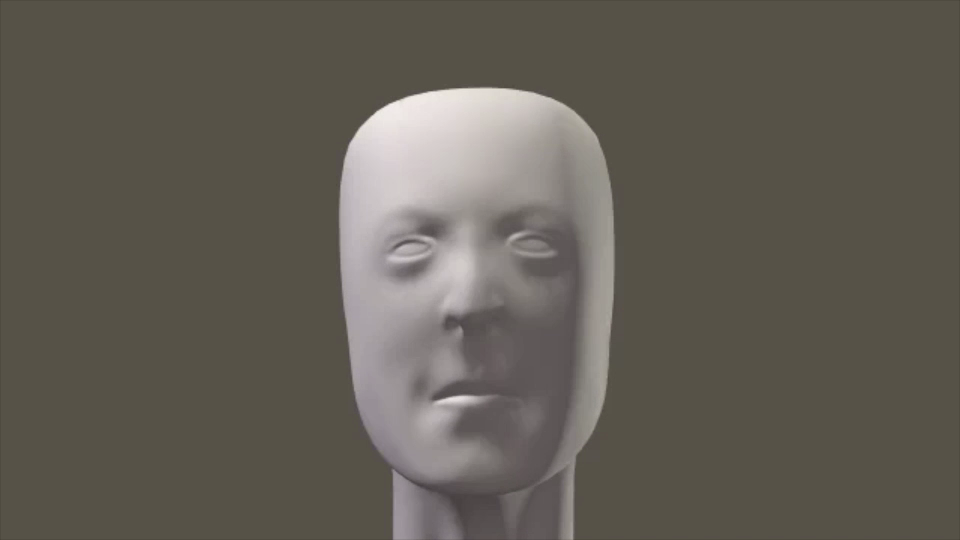
\includegraphics[width=.3\textwidth]{fightclub4.png}
	\caption{Frames from the random system visualisation}
\end{figure}

\section{Rule-Based System}

The Rule-Based system uses the output from Festival to apply manually written rules in order to synthesise head motions. Having considered the initial results of the previous two system the third built upon those ideas integrating with the rules derived from the multiple hypotheses outlined in chapter 3.

As there if not a 1 to 1 mappings between head motions and the words found in speech, the rule-based system removes stop words : words that are very common or are short function words like 'the', 'and' and 'which'. The system used the list of stop words from the NLTK library.

\subsection{Using the information from festival}
\subsubsection{Intionation}

Initially, the system was designed to store all of the information regarding the fundamental frequency (F0) from the Festival output. This was so that the system contained complete information about the intonation but this proved to be fairly complicated.
\begin{lstlisting}
151 id _113 ; f0 102.921 ; pos 0.22 ; 
\end{lstlisting}
F0 values were only available to the individual phonemes of each word, with only timing value to relate it back to where it belonged. In order to store all of the F0 values a lot of pre-processing was done to carefully assign each value to it's correct word in the proper order. During this pre-processing the system computing the minimum, maximum and average values for comparison.

However, the information was difficult to work with due to the need for excessive pre-processing and so the system used the ToBi intonation tags from the Festival output in order to alter head motions based on the intonation. The ToBi tags proved to be very useful as they represented an overview for the intonation so the pre processing was reduced significantly.

The ToBi tags were reduced down to solely their letter indicators 'L' and 'H' as their combination provided sufficient information regarding the intonation changes. For example, 'L\*-L' was reduced to 'LL'. Depending of the values of the ToBi tags a 'shift' value was added to the Euler angle change. If the tags were all 'L' a shift value was subtracted, similarly if the tags were all 'H', the shift value was added. 

However, if the two ToBi tags were different for that word, the previous value would be 'shifted' to match the pattern and the current value would be shifted with an extra value. The default shift value was 5.0 change in the Euler angle, with an Extra 2.0 in the case of 'L-H' tags or 'H-L'. The intonation changes affected only the Roll Euler angle which influenced nodding motions.

\subsubsection{Break Strength}

\begin{lstlisting}
pbreak BB; pbreak B; pbreak NB;
\end{lstlisting}

As nodding motions were found at the end of phrases and phrase boundaries, the system was design to reset the Roll angle back to it's origin on strong phrase boundaries. That being phrase break values of BB as they were the strongest. This simple rule produced good results as the synthesised nodding motions returned to first position upon finishing the video, showing that the avatar is done speaking.

\subsubsection{Uniqueness}

As outlined in the hypotheses the system should reflect lexical lookups of unique words by tilting the head. Head tilts are reflected by the Pitch Euler angle.

The system uses the NLTK to build a Frequency Distribution of all the words in the Brown corpus \cite{brown}. This is so that each word in the utterance can be compared against this Frequency Distribution to assign a uniqueness value to that word. The system assigns a positive or negative value of 3 if the word has a uniqueness score of less than 5. The uniqueness score is assigned by the 'query\_corpus' method that divides the number occurrences of the word in the Brown corpus by the number of the most common word.

%\begin{lstlisting}
%def query_corpus(word):
%	occur = float(brown_freq[word])
%	return ( occur / float(top_occurence) ) * 1000
%\end{lstlisting}
%	

\subsubsection{Sentiment Scaling}

The rule based system performs sentiment analysis on the utterance. As NLTK does not come with an in built sentiment classifier other options were considered. 

Sentiment Classifier \cite{senti_class} is a sentiment analysis tool based on NLTK and the SentiWordNet that assigns a positive and negative score to words in order to classify sentences.

- Talk about it more.

\begin{lstlisting}
>>> from senti_classifier import senti_classifier
>>> sentences = ['The movie was the worst movie', 
'It was the worst acting by the actors']
>>> pos_score, neg_score = senti_classifier.polarity_scores(sentences)
>>> print pos_score, neg_score
0 0
>>> 
\end{lstlisting}
The example shown above was a recreation of the example on the package's website. The sentences received scores that did not match the example on their website. This error was due to package constraints not being satisfied. Sentiment Classifier requires NLTK, Numpy and the SentiWordNet corpus. TextBlob \cite{text_blob} was an alternative that did not rely on such package constrains and was far more lightweight than Sentiment Classifier. It assigns a sentiment score to a string of text between 1 and -1, 1 being an extremely positive sentiment and -1 being an extremely negative sentiment. An example of TextBlob is presented below.

\begin{lstlisting}
>>> from textblob import TextBlob
>>> tb = TextBlob("I am very happy because of the nice weather")
>>> tb.sentiment
Sentiment(polarity=0.8, subjectivity=1.0)
\end{lstlisting}

TextBlob was chosen to analyse the sentiment in the rule based system. The information, both the actual sentiment and the polarity was added to the information dictionary for reference.

As outlined in the hypotheses, negation cannot be captured effectively using purely sentiment analysis, and can often be used in positive sentences. To account for these findings the system used the twitter negation corpus \cite{neg_corpus} which builds upon \cite{negation_corpus_1}\cite{negation_corpus_2} and contains a list of around 5000 negative words captured from social media platform Twitter.

To use this corpus NLTK's Plaintext Corpus reader was used to read in the text file and store in into a query-able format. When the system iterates over each word, the negation corpus is queried to determine if the word in the utterance is present in the negation corpus. If present, the Yaw angle that controls head shakes will be assigned to the value of 3.0 and the previous word's Yaw value is reduced by 3.0 to produce a shake motion. If not present the system assign a uniform random number from -1 to 1.

\subsection{Parametric Smoothing}

One of the drawbacks from the initial reviews of the random system was that Bezier smoothing does not look like natural head motions. Having compared the output from the random system to the data recordings, the videos seemed to be more sharp and discontinuous, initially while smoothing out toward the end of the motion. The observed effect was similar to that of a first order differential equation, commonly used in electronics to represent the power in a circuit. Rising very quickly to begin with but slowing and smoothing off before reaching the desire level of output. 

\begin{figure}
	\centering
	$$ Y =  K * (1 - e^{\sfrac{-t}{T}})$$
	\\
	K = Steady State Gain\\
	T = Time Constant\\
	t = time\\
	
	\caption{First Order Equation Definition} 
\end{figure}

The parametric smoothing system used the first order differential equation shown above the determine the curve between two points. The equation requires several parameters to generate the correct, which was calculated for each pair of points as shown in Figure 4.7. The Time Constant was set to a value of 4.0. The system builds the formula and calculates the y values for each point in between the two points passed into the method 'curve\_between\_points()'. This y values represents value of the Euler angle change.

\begin{figure}
	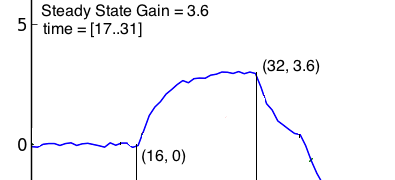
\includegraphics[width=0.9\textwidth]{parametric_ex.png}
	\caption{Graph showing Parametric smoothing between points.}
\end{figure}

The parametric smoothing provided good results and reflected the discontinuous nature of the recorded head motions.

% ============================================================= %
\chapter{Evaluation}

To evaluate the Text-Driven Head Motion System I performed both subjective analysis and objective analysis. The aim for the project was to develop a system which generates life-like talking heads with head motions that seem realistic and natural so it was important for humans to evaluate if the head motions were natural or not. Having a unit of measurement describing how close to the original head motions was also necessary in evaluating the system.

\section{Subjective Analysis}

\subsection{Design Overview}

The subjective evaluation was derived from the MUSHRA methodology outlined in chapter 2. It was designed with many factors taken into account. To effectively isolate the head motions for evaluations and make sure that participants were not affected or influenced by other factors, care was taken to ensure that as much as possible would remain constant, only changing the head motions.

Volunteers were shown 5 different video clips and were asked to evaluate how natural they felt the head motions were. Of the 5 videos, 3 were synthesised from the Text Driven Talking Heads system and 2 videos were taken from real recordings. Participants were not told anything about the videos and so did not know if the videos were synthesised or real. This was to eliminate any potential bias that could be introduced by telling the participants some of the videos were real and some were not and made sure that the participants focused on the task.

It was important for participants to be able to review their evaluation and update their choices as their subjective idea of what natural head motions are could easily change after watching the videos. Participants were encouraged to watch the videos more than once and update their evaluation are necessary until they were content with their evaluation.

The preliminary evaluation mapped the head motions to a character called 'Dom Casual' from the the Poser Standard Library as shown in figure 5.1.

As there had no be no indication which video was which, the video were simply labelled as number 1 through 5. The key is shown below.

\begin{description}
  	\item[Video 1]	Basic system
  	\item[Video 2] Desmond recordings
	\item[Video 3] Rule-based system
	\item[Video 4] Jane recordings
	\item[Video 5] Random system
\end{description}


\subsection{Implementation}

The evaluation platform was implemented in a web-based format using HTML5, Python and Flask, a Python framework used for web development. The website (shown in figure 5.1), showed the 5 videos side by side with sliders allowing the users to click and drag the slider to a level they felt reflected how natural the video above that slider was. This approach accomplished two things: having sliders ranging from 0 to 100 allowed for much greater precision than asking participants to rate the video from 1-5 or 1-10 and also helped users generate numeric feedback without the need to arbitrarily assign a numerical value.

As outlined in the design overview, only once participants were content with their evaluation would the results be recorded. The 'submit' button commits the users evaluation to a text file. This was suitable for the purpose of the evaluation system as it very simple to implement and had little development overhead.

\begin{figure}
	\centering
	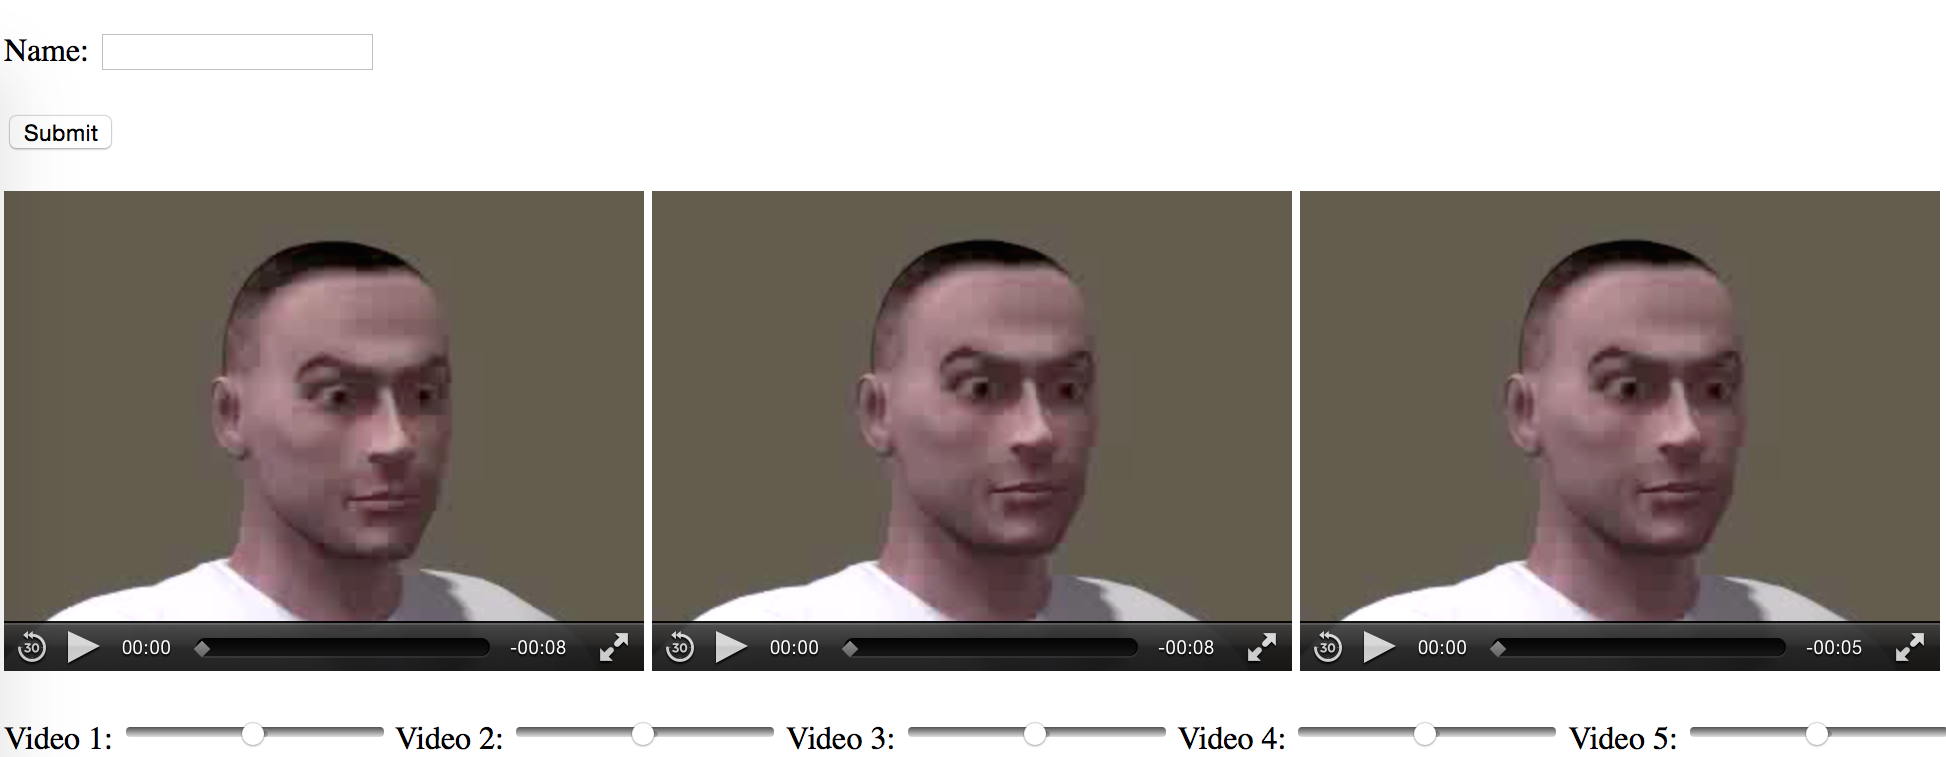
\includegraphics[width=1.0\textwidth]{eval_2.png}
	\caption{Preliminary Evaluation platform}
\end{figure}

\subsection{Preliminary feedback}

Preliminary evaluations were carried out to to test the evaluation platform. A small number of volunteers were asked to perform the evaluation and were asked a series of questions about the environment.

\begin{enumerate}
\item{How difficult was the task? What were the areas of difficulty?}
\item{Did you find the 3D avatars creepy?}
\item{Would the task be easier or more diffuclt with longer videos?}
\end{enumerate}

This was to try and improve the user experience before the final evaluation. The questions chosen were to address some key concerns regarding the environment. The participants were to feel comfortable during the evaluation process and if they videos they were evaluating were in the uncanny valley, many participants would feel discomfort which could negatively impact results. Gauging if participants felt the videos were too short or too long was important as well, the video needed to be of appropriate length so users had the right amount of information to effectively evaluate the videos.

The preliminary sessions provided good feedback on the system. Many participants stated that the avatar used for the videos was very distracting, particularly with the eyes of the avatar. Two of the six participants reported that they feel the avatar definitely influenced their evaluation. Participants reported that the length of the videos was suitable as they could re-watch the videos and re-evaluate the video.

\subsection{Final Evaluation}

Having taken on board the feedback from the preliminary results, the evaluation platform was tweaked. The head motion videos were re-exported from Poser with a different avatar. Rather than using a particular character from Poser Pro's library, the basic model called 'Andy' was used that lacks facial details like hair and appears as an emotionless manikin. This helped the participants focus solely on the head motions and not be distracted by the previous character's expression or facial features. The final subjective evaluation was performed on 15 participants.

\begin{figure}
	\centering
	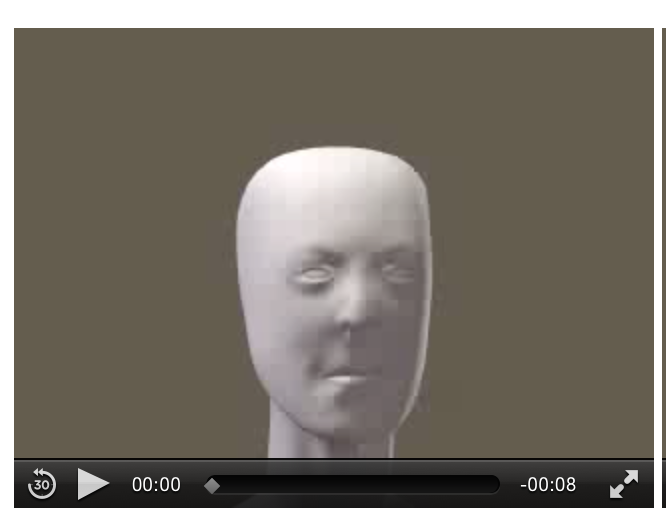
\includegraphics[width=0.6\textwidth]{eval_3.png}
	\caption{Avatar used for final Evaluation}
\end{figure}

\subsection{Results}

The subjective evaluation led to interesting results and results showed a  definite trend of which videos they felt were most natural. Interestingly, the head motions that were taken from recorded data were deemed to be fairly natural usually scoring around 60-70. These videos were added into the subjective evaluation as anchors for the evaluation and were intended to score highly but they scored less than expected. A possible reason for this could be that the recorded data does not necessarily align with what most people deem to be natural head motions.

The basic system that used a sine wave to generate a smooth nodding motion scored relatively well against the anchors, usually on par with one or both of the anchors. 

The rule based system was deemed un-natural by almost all of the participants. Many participants reported that the head motions were very 'jerky' and looked un-natural because of this. This does not necessarily mean that the hypotheses made regarding introducing more discontinuous head motions is incorrect and could be because parameters used for smoothing were not optimal.

The random system scored highest overall, including the videos taken from the data recordings. With no relation to the content of the text this is a very surprising result. 

\begin{figure}
	\centering
	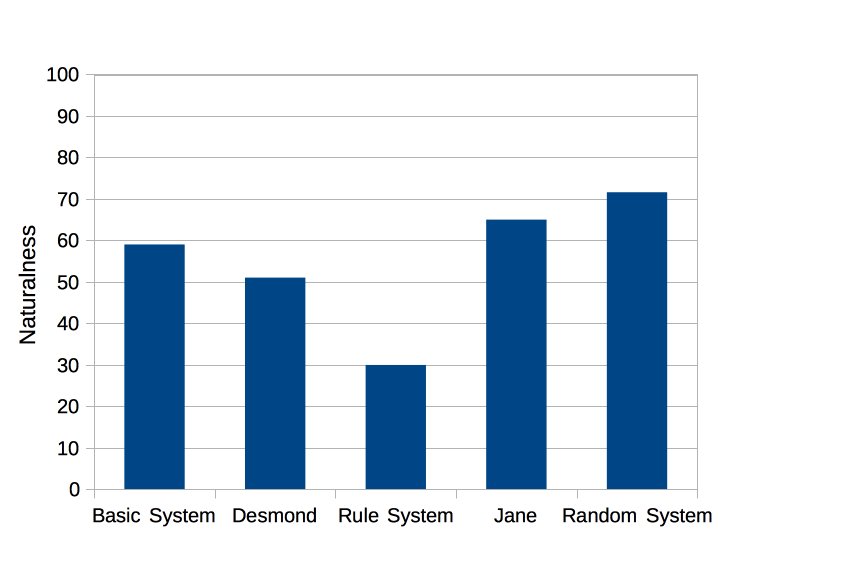
\includegraphics[width=1.0\textwidth]{chart.png}
	\caption{Mean 'naturalness' of each video}
\end{figure}

\subsection{Conclusions}

The main factor which seemed to influence how natural participants deemed the head motions was how smooth the head motions were. The rule based system performed poorly in the evaluation because of it's jerky, discontinuous nature and the random system scored very highly due to it's smooth motions. These results highlight a potential issue with the evaluation method: participants are given any information about the text the head motions were synthesised or taken from (in the case of the data recordings) and how the head motions relate to what is being said is not a factor. 

- low score because of environment

\section{Objective Analysis}

To evaluate the system objectively the output of a system was compared with both data recordings used for evaluation previously. The Euler angles were periodically sampled every 10 frames and the distance between the two head positions was calculated using the Euclidian distance measure. The values were then normalised using their sampling rate so that different sampling rates could be used and compared. The neutral position was also used for the objective evaluation, that being the point (0,0,0). The sampling rate used for the objective evaluation was every 10th frame. 

$$ Euclidian(x,y) = \sqrt{(x1 - y1)^2 + (x2 - y2)^2 + ... + (x_n - y_n)^2}$$

\subsection{Results}

\begin{table}[h]
\begin{tabular}{lllll}
\hline
Euler Distance & Origin & Sine  & Random & Rule   \\ \hline
Desmond        & 6.3    & 7.02  & 6.4    & 6.94   \\
Jane           & 17.68  & 18.08 & 18.8   & 18.6 \\ \hline
\end{tabular}
\end{table}

The results from the objective evaluation show that the two head motions that are most similar in terms of raw distance measure are that of the origin (no Euler change) and the Desmond Euler angles. The distance between the head position and the origin was seemed to be a large factor when comparing the distance. The distance between Desmond and the origin is very close to the distance between Desmond and all the synthesised motions and the same is true for Jane. 

The approach taken to measure the head motion similarity is naive, and does not take into account the possibility of head motions being very similar in gesture like a nod but having a low score because of a large distance in the other Euler angles due to tilts and shakes present in the head motions.



% ============================================================= %

\chapter{Conclusions}



\section{System Overview}

\section{Discussion}

\subsection{Classification and Regression Trees}

\subsection{Data Driven System}

\section{Future Work}

\subsection{Expansion of techniques}

\subsection{Second Order Smoothing}
	
\bibliographystyle{plain}
\bibliography{diss}

\end{document}
